\section{Introduction}
\label{sec:intro}

\begin{figure}[!t]
  \centering
  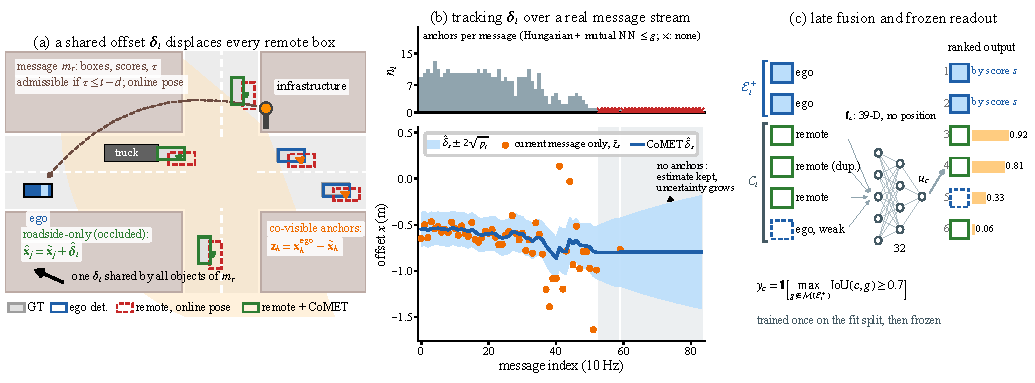
\includegraphics[width=\linewidth]{fig/overview.pdf}
  \caption{\textbf{\method at a glance.}
  (a)~A roadside message is admissible only if it was captured at least $d$\,ms before the decision time $t$. Placed with online poses, all remote boxes (red, dashed) are displaced from the ground truth (gray) by the same offset $\boldsymbol\delta_t$ (exaggerated here). Objects seen by both agents yield anchor residuals $\mathbf z_k$ between ego boxes (blue) and remote boxes that measure $\boldsymbol\delta_t$; the tracked estimate moves every remote box, including the roadside-only objects hidden behind the truck (green).
  (b)~A real validation stream (sequence 0071, $d=0$). Anchors per message come from Hungarian matching of all ego detections with a mutual-nearest-neighbour gate. The estimate from the current message alone (orange) is noisy and absent when there are no anchors (gray bands); the \method estimate (blue) is stable, is kept through anchor-free messages and its uncertainty grows until anchors return.
  (c)~Confident ego detections form a protected prefix $\mathcal E^+_t$; corrected remote boxes and weak ego boxes $\mathcal C_t$ are ranked by a 1.3K-parameter readout head on 39 receiver-side features without absolute position, trained once and frozen. Only boxes, scores and capture times are transmitted.}
  \label{fig:overview}
\end{figure}


An ego vehicle approaching an intersection cannot see the car hidden behind a truck; a LiDAR mounted on a pole above the intersection can.
Telling the vehicle where that car is, early enough to plan around it, is the promise of vehicle--infrastructure (V2I) cooperative perception~\cite{yu2022dairv2x,yu2023v2xseq}.
Most methods fuse the two views at the feature level~\cite{chen2019fcooper,wang2020v2vnet,li2021disconet,xu2022v2xvit,hu2022where2comm,xu2022cobevt} or at the box level~\cite{yu2022dairv2x}, and most reported gains are measured with views that are synchronised and registered with carefully calibrated poses.

A deployed receiver has neither.
The roadside message was captured before the ego frame and arrives after a communication delay, and it can only be placed with the poses that are available online: the vehicle's localisation estimate and the roadside calibration.
We evaluate V2X-Seq~\cite{yu2023v2xseq} under a \emph{strict arrival protocol} that admits only messages captured at least $d$\,ms before the decision time ($d\in\{0,100,200,400\}$) and that never uses ground truth, future frames or the dataset's per-pair calibration offsets at inference.
Under this protocol, cooperation as currently practised adds little (\cref{fig:latency}): late fusion with online poses raises \apseven over the ego detector by 1.0 point, and three intermediate-fusion models change it by $-1.0$ to $+0.8$.
Yet the value is there: the same late fusion placed with the dataset's annotation-assisted offsets would raise \apseven by 7.4 points.
The decisive limitation is therefore geometric, not temporal.

\paragraph{The error is shared, persistent and sparsely observed.}
V2X-Seq provides one planar translation per frame pair, and applying it recovers most of the lost accuracy; a single translation shared by all objects of a message---a \emph{common-mode} error---therefore explains most of the misplacement.
This error is observable without any label: an object seen by both agents (an \emph{anchor}) yields a residual between the ego box and the projected roadside box that measures the shared translation, and the same correction then applies to the roadside-only objects that motivate cooperation in the first place.
A single message, however, carries little evidence.
On the validation sequences a message holds 2.96 anchors on average, and 38\% of messages hold none; estimates from the current message alone are therefore often impossible and, when possible, noisy (a radial error of 0.48\,m against a smoothed reference at 0\,ms and 0.61\,m at 400\,ms).
At the same time the error drifts slowly within a sequence (\cref{fig:trajectory}).
The misalignment is a property of the \emph{message stream}, not of any individual frame.

\paragraph{Tracking instead of registering.}
Latency-aware methods~\cite{lei2022syncnet,wei2023cobevflow,yu2023ffnet,yang2023how2comm,song2025trafalign} compensate motion between capture and use and assume that the relative pose is right.
Pose-robust methods~\cite{lu2023coalign,lei2024freealign,huang2024roco,song2023cbm} re-register each frame from its own correspondences and are mostly evaluated under independent synthetic noise.
Neither treats the partner's error as persistent: the first leaves it uncorrected, and the second re-estimates it from scratch in every frame, so no estimate is available when correspondences are missing.
We propose \method (Common-Mode Error Tracking), which treats the partner's current systematic error as a state to be estimated together with its uncertainty.
\method uses every ego detection as an anchor candidate, forms one robust observation per message with mutual-nearest-neighbour Hungarian matching, tracks the shared offset with a causal Kalman filter per sender, carries the estimate through messages without anchors, and transfers it to every remote box (\cref{fig:overview}).
When the offset is larger than the association gate, a lock-acquisition step recovers it from a vote over the displacements of recent messages.
A small frozen readout head then re-ranks the corrected boxes together with the low-score ego detections.
Because process and measurement noise are isotropic, the filter reduces exactly to a scalar recursion with a two-coordinate state and one variance per stream; it has no learned parameters and needs only the boxes that a late-fusion message already carries.
Its two limiting cases are the two classical answers to pose error, per-frame registration and fixed calibration, and on real data it outperforms both.

\paragraph{The benchmark's reference is itself incomplete.}
Evaluating such a method requires care, because the reference offsets of V2X-Seq are not what they appear to be.
We audit them against the raw annotations and find that (i) the offset is \emph{exactly zero} on 28.0\% of validation messages, nearly all of which contain no co-labelled object, so zero is a placeholder rather than a measurement; (ii) the roadside-only ground truth is the public projection plus this offset (residual $\approx4\times10^{-7}$\,m), so on placeholder frames the ground truth itself is uncorrected; and (iii) the non-zero offsets come from a bounded discrete search with 26 values per axis whose bound is reached on 44.6\% of non-zero validation messages, where the co-labelled objects are typically displaced beyond the bound (\cref{fig:audit}).
An estimator that is right on a placeholder frame is therefore penalised by the official evaluation, and the dataset offset is a label-consistent reference rather than an oracle.
We report the official evaluation as the primary result and complement it with label-defined populations and two auxiliary references; under both auxiliary references \method improves on every population.

\paragraph{Results.}
With the boxes of the released TraF-Align detector, \method reaches 66.63 \apseven averaged over the four latency budgets, 3.45 points above late fusion with online poses and 3.67 above the best intermediate fusion, while keeping the advantage at every budget.
It improves the late fusion of all five detectors we test by 2.2--3.5 points over online poses and by 0.3--0.6 over estimating the offset from the current message alone. Nine variants of three per-frame registration modules, with and without temporal smoothing, remain 2.3--3.1 points behind, and as the pose input of CoAlign, \method beats CoAlign's own pose graph by 1.1 points.
With known pose errors of 3--5\,m injected into the roadside messages, \method with lock acquisition keeps 97.6--99.5\% of its accuracy for all five detectors, and its corrected pose raises the accuracy of retrained intermediate fusion under the same errors by 2.2--4.4 points.
When intermediate fusion is retrained, using \method poses and cleaned labels is better than retraining with online poses on all three architectures we test (significantly on two).
Combining the boxes of the retrained network with those of \method late fusion reaches 67.85 \apseven and 82.62 \apfive, better than either alone on both metrics.

\paragraph{Contributions.}
\begin{itemize}
  \item We show that under strict arrival and online poses the main obstacle to real V2I cooperative detection is a slowly drifting common-mode translation, which co-visible objects reveal but which no single message estimates reliably.
  \item We propose \method, a training-free causal tracker of this translation with cross-object transfer, which interpolates between per-frame registration and fixed calibration, re-acquires offsets beyond its association gate, and costs a single small assignment per message.
  \item We audit the reference offsets of V2X-Seq, identify a zero placeholder and a saturated bounded search, explain how they enter the official ground truth, and propose an evaluation that separates label artefacts from method effects.
  \item We provide an extensive evaluation with paired sequence-level confidence intervals, hyper-parameters selected on a separate calibration split only, every reported number re-derived by an independent implementation, a controlled study with injected pose errors on real data, and a retraining study across three architectures together with a box-level combination of late and intermediate fusion.
\end{itemize}

